\subsection{Заготовка шаблона}
Воспользуемся заготовкой шаблона приведенной ниже. Код заготовки поставляется вместе с программой генератором и этой документацией.

\begin{figure}[H]
\lstinputlisting{docExamples/templateExample1.lua}
\caption{Заготовка для создания шаблона \texttt{example.lua}}
\end{figure}

Разберем текст заготовки подробно:\\
Наш шаблон будет создавать сценарии размером от 48 до 72, на выбор игрока:
\begin{figure}[H]
\lstinputlisting[firstnumber=4, firstline=4, lastline=5]{docExamples/templateExample1.lua}
\end{figure}

Наш шаблон будет создавать сценарии для двух игроков:

\begin{figure}[H]
\lstinputlisting[firstnumber=6, firstline=6, lastline=6]{docExamples/templateExample1.lua}
\end{figure}

По-умолчанию процент лесов 65:

\begin{figure}[H]
\lstinputlisting[firstnumber=7, firstline=7, lastline=7]{docExamples/templateExample1.lua}
\end{figure}

Также, на 40\% клеток проходов будут созданы тайлы дорог, дающие бонус наземным отрядам:

\begin{figure}[H]
\lstinputlisting[firstnumber=8, firstline=8, lastline=8]{docExamples/templateExample1.lua}
\end{figure}

Бонус по стартовому золоту для обоих игроков по-умолчанию задан в 850:

\begin{figure}[H]
\lstinputlisting[firstnumber=9, firstline=9, lastline=9]{docExamples/templateExample1.lua}
\end{figure}

Функция \texttt{getContents} возвращает таблицу содержающую список из двух зон:

\begin{figure}[H]
\lstinputlisting[firstnumber=13, firstline=13, lastline=26]{docExamples/templateExample1.lua}
\end{figure}

Первая зона в списке имеет \texttt{id} 0. Используя этот номер мы затем сможем задать проход между зонами:

\begin{figure}[H]
\lstinputlisting[firstnumber=15, firstline=15, lastline=15]{docExamples/templateExample1.lua}
\end{figure}

Первая зона является стартовой зоной игрока, там будет расположена столица:

\begin{figure}[H]
\lstinputlisting[firstnumber=16, firstline=16, lastline=16]{docExamples/templateExample1.lua}
\end{figure}

Расы игроков будут выбраны самими игроками перед началом генерации по шаблону, мы лишь определяем что первая раса из списка рас будет стартовать в этой зоне:

\begin{figure}[H]
\lstinputlisting[firstnumber=17, firstline=17, lastline=17]{docExamples/templateExample1.lua}
\end{figure}

Первая зона будет иметь относительный размер равный половине размера сценария. В зависимости от выбора игрока, размер сценария будет либо 48, либо 72, согласно нашим ограничениям на доступные размеры. Зона будет масштабирована с учетом размеров сценария.

\begin{figure}[H]
\lstinputlisting[firstnumber=18, firstline=18, lastline=18]{docExamples/templateExample1.lua}
\end{figure}

Поскольку размеры зон являются относительными значениями, нам важно отношение размеров двух зон. Поскольку размеры двух зон одинаковы, каждая будет занимать от 50\% площади карты. Можете поиграть меняя размеры зон относительно друг друга и наблюдать результаты генерации, только не проиграйте.

\begin{figure}[H]
\lstinputlisting[firstnumber=18, firstline=18, lastline=18]{docExamples/templateExample1.lua}
\lstinputlisting[firstnumber=24, firstline=24, lastline=24]{docExamples/templateExample1.lua}
\end{figure}

Вторая зона в списке имеет \texttt{id} 1:

\begin{figure}[H]
\lstinputlisting[firstnumber=21, firstline=21, lastline=21]{docExamples/templateExample1.lua}
\end{figure}

Вторая зона также является стартовой зоной, там будет расположена столица:

\begin{figure}[H]
\lstinputlisting[firstnumber=22, firstline=22, lastline=22]{docExamples/templateExample1.lua}
\end{figure}

Вторая раса из списка рас будет стартовать во второй зоне:

\begin{figure}[H]
\lstinputlisting[firstnumber=23, firstline=23, lastline=23]{docExamples/templateExample1.lua}
\end{figure}

Помимо двух зон, таблица содержит список проходов между зонами, в нашем случае зоны соединены одним проходом. Здесь поля \texttt{from} и \texttt{to} ссылаются на идентификаторы зон.

\begin{figure}[H]
\lstinputlisting[firstnumber=28, firstline=28, lastline=30]{docExamples/templateExample1.lua}
\end{figure}

\subsubsection{Проверка заготовки}
Проверим что наша заготовка шаблона корректна, сгенерировав карту.

Выбираем мод и загружаем шаблон в программу:

\begin{figure}[H]
\center
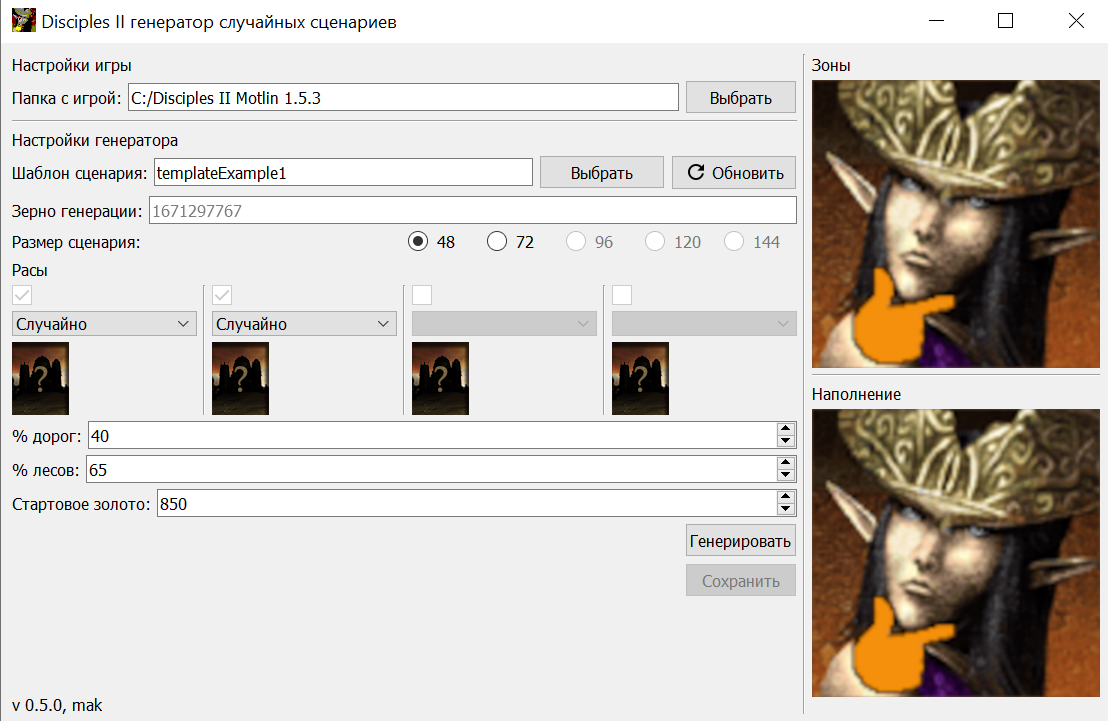
\includegraphics[width=.8\linewidth]{docImages/exampleTemplateLoaded.png}
\caption{Программа генератора с загруженным шаблоном}
\end{figure}

Убедимся что наши дефолтные настроки видны программе и отображены корректно: доступные размеры сценариев, две расы, \% лесов и дорог, стартовое золото.\\
Жмем кнопку \texttt{"Генерировать"} для генерации сценария по шаблону с учетом настроек:

\begin{figure}[H]
\center
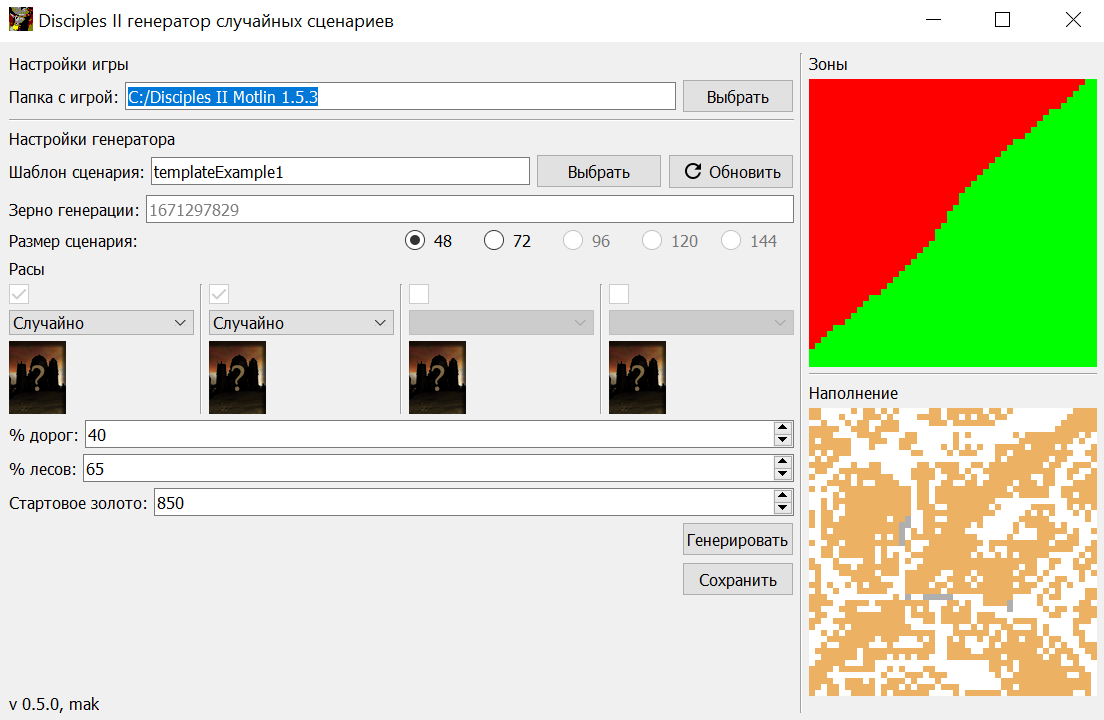
\includegraphics[width=.8\linewidth]{docImages/scenarioGenerated.png}
\caption{Программа с результатами генерации}
\end{figure}

Справа, в окне предпросмотра, видим как карту поделило на две зоны с разными цветовыми индикаторами. В просмотре наполнения видим свободные белые клетки, занятые золотые клетки и клетки дорог, дающие бонус движения, помеченные серым цветом.

Сохраняем сценарий в папку \texttt{Exports} мода, который был выбран и смотрим результаты в редакторе:

\begin{figure}[H]
\center
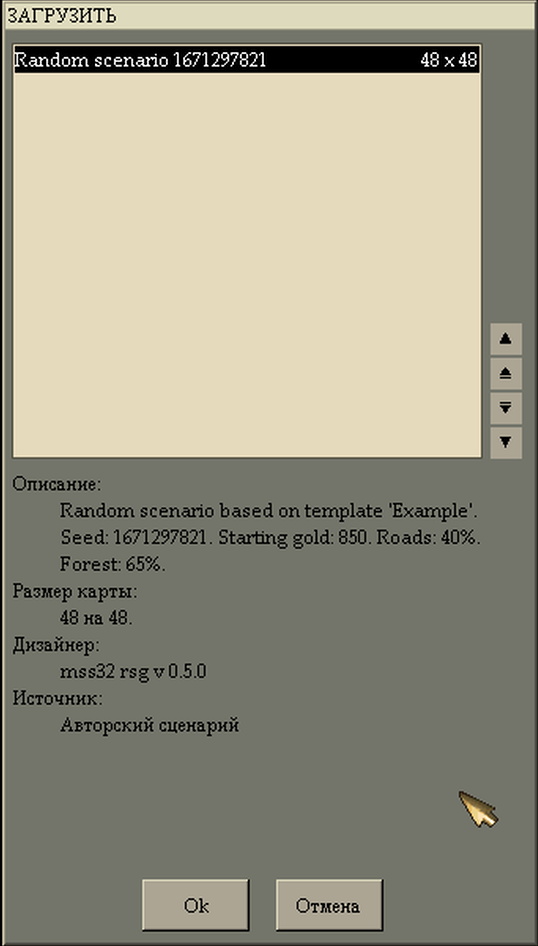
\includegraphics[width=.48\linewidth]{docImages/scenarioInEditor.png}
\caption{Сгенерированный сценарий в редакторе карт}
\end{figure}

Открываем сценарий и смотрим глобальную карту, а также мини-карту:

\begin{figure}[H]
\center
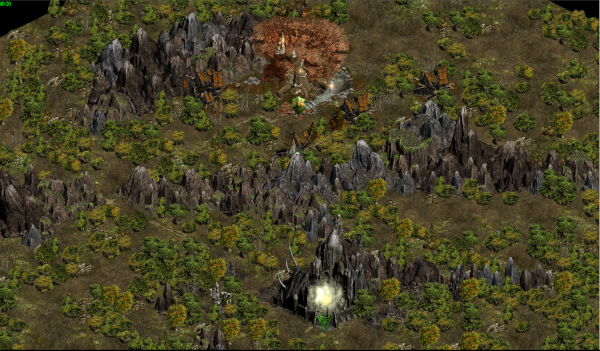
\includegraphics[width=1.0\linewidth]{docImages/scenarioMap.png}
\caption{Случайная карта в редакторе}
\end{figure}

\begin{figure}[H]
\center
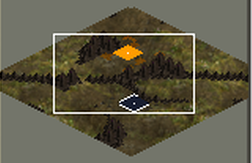
\includegraphics[width=.48\linewidth]{docImages/scenarioMinimap.png}
\caption{Миникарта}
\end{figure}

Убеждаемся что результаты совпадают с описанием в шаблоне: два игрока, каждый в своей зоне. Зоны соединены одним проходом. Поскольку при генерации были выбраны случайные расы, генератор выбрал для сценария Эльфов и Орды нежити.